%++++++++++++++++++++++++++++++++++++++++
% Don't modify this section unless you know what you're doing!
\documentclass[letterpaper,12pt]{article}
\usepackage{authblk}
\usepackage{tabularx} % extra features for tabular environment
\usepackage{amsmath, amssymb}  % improve math presentation
\usepackage{amsfonts}
\usepackage{graphicx} % takes care of graphic including machinery
\usepackage[margin=1in,letterpaper]{geometry} % decreases margins
\usepackage{cite} % takes care of citations
\usepackage[final]{hyperref} % adds hyper links inside the generated pdf file
\hypersetup{
    colorlinks=true,       % false: boxed links; true: colored links
    linkcolor=blue,        % color of internal links
    citecolor=blue,        % color of links to bibliography
    filecolor=magenta,     % color of file links
    urlcolor=blue         
}
\usepackage{float}
\usepackage{listings}
\usepackage[titletoc,title]{appendix}
\usepackage{siunitx}
\usepackage[table]{xcolor}
\setcounter{MaxMatrixCols}{30}
\usepackage{bm}
\newcommand{\myMatrix}[1]{\bm{\mathit{#1}}}

\newcommand{\nuc}[2]{$^{#2}$#1}
%++++++++++++++++++++++++++++++++++++++++

\begin{document}
\title{My Favorite Least Squares Fitting Tricks \\ (rough draft, not for distribution)}
\author{Charles Whitmer}
%\affil{TerraPower LLC, Bellevue, Washington, USA}
\date{\today}
\maketitle

\begin{abstract}
Over the years I have performed thousands of least squares fits, and written software in several languages to calculate those fits. I've got a simple way of looking at things that some people might find useful.
\end{abstract}

\section{Linear Least Squares}
\label{sec.one}
Suppose we have a set of independent variables $x_i$ and related observations $y_i$. The first fit we will look at will try to find a linear relationship between $x$ and $y$, specifically, the best $a$ and $b$ for the model $y=ax+b$. To find these we will minimize the sum of squares $S^2$ over all possibilities for $a$ and $b$:

\begin{equation} \label{S.square}
S^2=\sum_{i=1}^N (a x_i + b - y_i)^2
\end{equation}

The solution is found easily by taking derivatives of $S^2$ and setting them to $0$:

\begin{equation}
\begin{aligned}
\frac{\partial}{\partial a}S^2&=2\sum_{i=1}^N x_i(a x_i+b-y_i)=0\\
\frac{\partial}{\partial b}S^2&=2\sum_{i=1}^N (a x_i+b-y_i)=0
\end{aligned}
\end{equation}

We can rearrange this into two linear equations in two variables.

\begin{equation}
\begin{aligned}
\label{linear1}
\sum_{i=1}^N a x_i^2+b x_i &= \sum_{i=1}^N x_i y_i\\
\sum_{i=1}^N a x_i+b &= \sum_{i=1}^N y_i
\end{aligned}
\end{equation}

Since all the $x_i$ and $y_i$ are known, this consists only of $a$, $b$, and a bunch of constants, and so it is a simple problem in linear algebra.

Actually, the name ``Linear Least Squares'' does not refer to the linear model that we are fitting, instead it refers to the fact that the problem reduces to a set of linear equations in our unknown parameters, as in (\ref{linear1}). We will expand on this later.

Also, especially looking forward to more complex models, I have found a particular notation useful in solving Linear Least Squares problems. Suppose I define ``twiddle'' parameters as follows:

\begin{equation}
\begin{aligned}
\label{twiddle1}
\widetilde{x}&=\sum_{i=1}^N x_i\\
\widetilde{xx}&=\sum_{i=1}^N x_i^2\\
\widetilde{y}&=\sum_{i=1}^N y_i\\
\widetilde{xy}&=\sum_{i=1}^N x_i y_i\\
\widetilde{1}&=\sum_{i=1}^N 1=N
\end{aligned}
\end{equation}

It is important to keep in mind that $\widetilde{1}$ is not $1$, but $N$ in this case. 

We can now rewrite (\ref{linear1}) in matrix form:

\begin{equation}
\begin{pmatrix}
\widetilde{xx} & \widetilde{x} \\
\widetilde{x} & \widetilde{1}
\end{pmatrix}
\begin{pmatrix}
a \\
b
\end{pmatrix} =
\begin{pmatrix}
\widetilde{xy}  \\
\widetilde{y}
\end{pmatrix}
\end{equation}

And so the solution is:

\begin{equation}
\begin{pmatrix}
a \\
b
\end{pmatrix} =
\begin{pmatrix}
\widetilde{xx} & \widetilde{x} \\
\widetilde{x} & \widetilde{1}
\end{pmatrix} ^{-1}
\begin{pmatrix}
\widetilde{xy}  \\
\widetilde{y}
\end{pmatrix}
\end{equation}

\section{A Better Way to do Things}

The above can be generalized to more complicated models, but first it is important to note that our simple definition of $S^2$ is not very useful. All of the data points in our fit have been given the same weight, when in real life that would usually not be the case. In most experiments, some data points are more accurate than others, and that should be reflected in our best fit.

The solution is to modify equation (\ref*{S.square}) to instead read:

\begin{equation} \label{chi.square}
\chi^2=\sum_{i=1}^N \frac{(a x_i + b - y_i)^2}{\sigma_i^2}
\end{equation}
where $\sigma_i$ is the standard deviation (i.e. ``error'') of the measurement $y_i$.

Obviously, when a $y_i$ value is more accurately determined, the $\sigma_i$ is smaller and then the $\sigma_i^2$ in the denominator gives a larger contribution to the sum. In order to minimize $\chi^2$ we are going to have to fit the points with small measurement errors more closely.

Note also that $\sigma_i$ carries the same units as $y_i$, and that the sum will therefore be dimensionless. It turns out that if the model is a good one, and the $\sigma_i$ values are reasonable, then the resulting minimal value of $\chi^2$ will follow what is know as the chi-square distribution. 

Each time you run your experiment and get new $y_i$ values, your best fit will change slightly and you will get a new $\chi^2$ value. You could repeat this process many 
times and histogram the $\chi^2$ values. In this sense it is a distribution.

\section{Degrees of Freedom}
The chi-square distribution is well known, but is actually a set of distributions enumerated by $k$, the number of ``degrees of freedom''.

Suppose we perform an experiment and measure 10 values of $y_i$. The set of results can vary in a 10-dimensional space, and we would call that 10 degrees of freedom. When we fit this data to a linear model, i.e. one with two parameters, we would hope to take away two degrees of freedom from the residuals (the differences between the data and the best fit) and we would say that 8 degrees of freedom would be left over. The best fist found from minimizing equation (\ref{chi.square}) would give a $\chi^2$ value that should follow a chi-square distribution with 8 degrees of freedom. We can look up the value in a table of the chi-square distribution for 8 degrees of freedom and read out how probable that result is. (At least in the old days I would do that. A good scientific calculator these days should have the function built in. On the HP-Prime you would use {\footnotesize CHISQUARE\_CDF}; on the TI-84 the function is $\chi^2$cdf.)

It happens that the mean value of the chi-square distribution for $k$ degrees of freedom is exactly $k$. So when we do our experiment measuring our 10 data points and then fit them to a linear model, we would hope that the minimum $\chi^2$ would be about 8. If it is far off from that, then either the model or our error estimates are bad.

To try to develop an intuition about the degrees of freedom, suppose we did an experiment taking two data points, and then fit a linear model to it. Well, we can perfectly fit a line to any two data points, so our $\chi^2$ value would be zero. This is a poor experiment because we have no degrees of freedom left to judge how good the fit is. If we had taken 3 data points to test our linear model, then we would have one degree of freedom to test, and we would hope to get a $\chi^2$ value around 1 for a successful fit.

\section{A Linear Model Using $\chi^2$}
Let's revisit the fit of the linear model that we did in section \ref*{sec.one}. If you work through the math you will see that we simply need to redefine the twiddle variables like this:

\begin{equation}
\begin{aligned}
\label{twiddle2}
\widetilde{x}&=\sum_{i=1}^N \frac{x_i}{\sigma_i^2}\\
\widetilde{xx}&=\sum_{i=1}^N \frac{x_i^2}{\sigma_i^2}\\
\widetilde{y}&=\sum_{i=1}^N \frac{y_i}{\sigma_i^2}\\
\widetilde{xy}&=\sum_{i=1}^N \frac{x_i y_i}{\sigma_i^2}\\
\widetilde{1}&=\sum_{i=1}^N \frac{1}{\sigma_i^2}
\end{aligned}
\end{equation}

And now note that $\widetilde{1}$ is not even $N$, but something complicated, so beware when manipulating it.

Given the new twiddle definitions, the solution looks identical:

\begin{equation} \label{eq.linear.solution}
\begin{pmatrix}
a \\
b
\end{pmatrix} =
\begin{pmatrix}
\widetilde{xx} & \widetilde{x} \\
\widetilde{x} & \widetilde{1}
\end{pmatrix} ^{-1}
\begin{pmatrix}
\widetilde{xy}  \\
\widetilde{y}
\end{pmatrix}
\end{equation}

However, what we have now is a better result, and it required no more complexity.

\section{More Interesting Models}
What happens when we get more complicated than a linear model? Let's try a cubic model:

\begin{equation}
y=a x^3 + b x^2 + c x + d
\end{equation}

You can work through the math, which is again easy, but here is the solution expressed in twiddle notation:

\begin{equation} \label{eq.cubic.solution}
\begin{pmatrix}
a \\
b \\
c \\
d
\end{pmatrix} =
\begin{pmatrix}
\widetilde{x^6} & \widetilde{x^5} & \widetilde{x^4} & \widetilde{x^3} \\
\widetilde{x^5} & \widetilde{x^4} & \widetilde{x^3} & \widetilde{x^2} \\
\widetilde{x^4} & \widetilde{x^3} & \widetilde{x^2} & \widetilde{x} \\
\widetilde{x^3} & \widetilde{x^2} & \widetilde{x} & \widetilde{1} 
\end{pmatrix} ^{-1}
\begin{pmatrix}
\widetilde{x^3y}  \\
\widetilde{x^2y}  \\
\widetilde{xy}  \\
\widetilde{y}
\end{pmatrix}
\end{equation}

There is an obvious pattern to this, and it holds to all orders.

Once you have used this a few times, it becomes obvious and you can write it from memory. More than once I have written a polynomial fit routine in some computer language and not even needed notes. You simply sum up the twiddle parameters in a loop, arrange them in a matrix, and then call your favorite matrix inverter or linear equation solver.

Models that look even more complex can be solved, i.e. fit, in this way. For example, last year I needed a fit to this model:

\begin{equation} \label{eq.sincosmodel}
y = a\ sin(\omega t)+ b\ cos(\omega t)+c\ t + d
\end{equation}
I knew the value of $\omega$ already, so this model is just linear in four unknowns, and therefore I could use linear least squares. By defining more twiddle variables, the solution can be quickly written:

\begin{equation} \label{eq.sincos}
\begin{pmatrix}
a \\
b \\
c \\
d
\end{pmatrix} =
\begin{pmatrix}
\widetilde{sin\ sin} & \widetilde{sin\ cos} & \widetilde{t\ sin} & \widetilde{sin} \\
\widetilde{sin\ cos} & \widetilde{cos\ cos} & \widetilde{t\ cos} & \widetilde{cos} \\
\widetilde{t\ sin} & \widetilde{t\ cos} & \widetilde{t^2} & \widetilde{t} \\
\widetilde{sin} & \widetilde{cos} & \widetilde{t} & \widetilde{1} 
\end{pmatrix} ^{-1}
\begin{pmatrix}
\widetilde{y\ sin}  \\
\widetilde{y\ cos}  \\
\widetilde{y\ t}  \\
\widetilde{y}
\end{pmatrix}
\end{equation}

I can be as casual as I like with the notation, as long as it comes back to a rigorous definition:

\begin{equation}
\begin{aligned}
\label{twiddle3}
\widetilde{sin\ sin}&=\sum_{i=1}^N \frac{sin^2(\omega t_i)}{\sigma_i^2}\\
\widetilde{sin\ cos}&=\sum_{i=1}^N \frac{sin(\omega t_i)cos(\omega t_i)}{\sigma_i^2}\\
\widetilde{t\ sin}&=\sum_{i=1}^N \frac{t_i sin(\omega t_i)}{\sigma_i^2}\\
\widetilde{y\ sin}&=\sum_{i=1}^N \frac{y_i sin(\omega t_i)}{\sigma_i^2}\\
\end{aligned}
\end{equation}
and so on.

Take a moment to look at the pattern of the matrix in equation (\ref{eq.sincos}). The parameters $a$, $b$, $c$, $d$ multiply the functions $sin(\omega t)$, $cos(\omega t)$ $t$, and $1$ in the model (\ref{eq.sincosmodel}). Since $a$ multiplies the $sin(\omega t)$, the first line of the matrix multiplies the $sin$ by each of the four functions. In the second line, the $cos$ multiplies each of the functions, and so on. This is obvious if you think of the derivatives that lead to this.

Also note that the matrix is always symmetric. This is a good thing to check.

\section{Bonus: The Covariance of the Fit}

I call this a bonus, because while any statistics course will teach you how to solve linear least squares problems, they almost never cover this part.

Suppose you have fit some data to a cubic according to equation (\ref{eq.cubic.solution}).  Now suppose somebody asks you what the error bars are on your resultant parameter $a$.  How would you know?

One way to get the error on $a$ is through the usual method of error propagation. Specifically, if $a=f(y_1,y_2,...,y_N)$ then 

\begin{equation}
\sigma_a^2=\sum_{i=1}^N \sigma_i^2(\frac{\partial f}{\partial y_i})^2
\end{equation}
as long as the errors on each $y_i$ are independent.

We have such a dependence of $a$ on the set of $y_i$, and so we can do the calculation.  But wait!  If we have already calculated the matrix inverse in equation (\ref{eq.cubic.solution}), then just call it $\myMatrix{C}$,
\begin{equation}
\myMatrix{C}=\begin{pmatrix}
\widetilde{x^6} & \widetilde{x^5} & \widetilde{x^4} & \widetilde{x^3} \\
\widetilde{x^5} & \widetilde{x^4} & \widetilde{x^3} & \widetilde{x^2} \\
\widetilde{x^4} & \widetilde{x^3} & \widetilde{x^2} & \widetilde{x} \\
\widetilde{x^3} & \widetilde{x^2} & \widetilde{x} & \widetilde{1} 
\end{pmatrix} ^{-1}
\end{equation}
and this $\myMatrix{C}$ just happens to be the covariance matrix of the best fit parameters. (The proof involves only a bit of linear algebra.)

And now it is easy to pick out:
\begin{equation}
\begin{aligned}
\sigma_a&=\sqrt{\myMatrix{C}_{11}} \\
\sigma_b&=\sqrt{\myMatrix{C}_{22}} 
\end{aligned}
\end{equation}
and so on.

But having the covariance matrix is even more powerful than that. Suppose that, having done the fit, you need to report some function $g(a,b,c,d)$. What is the error on that calculated value? The answer comes from the covariance matrix:
\begingroup
\renewcommand*{\arraystretch}{1.5}
\begin{equation}
\sigma_g^2=
\begin{pmatrix}
\frac{\partial g}{\partial a} &\frac{\partial g}{\partial b} &\frac{\partial g}{\partial c} &\frac{\partial g}{\partial d} 
\end{pmatrix}
\myMatrix{C}
\begin{pmatrix}
\frac{\partial g}{\partial a} \\
\frac{\partial g}{\partial b} \\
\frac{\partial g}{\partial c} \\
\frac{\partial g}{\partial d} 
\end{pmatrix}
\end{equation}
\endgroup

To make this more concrete, suppose we have fit our data to the linear model $y=ax+b$ and what is important to us is not simply $a$ or $b$, but the x-intercept. The x-intercept is obviously:

\begin{equation}
x_0=-\frac{b}{a}
\end{equation}

Assume we have calculated:
\begin{equation}
\myMatrix{C}_{linear}=
\begin{pmatrix}
\widetilde{xx} & \widetilde{x} \\
\widetilde{x} & \widetilde{1}
\end{pmatrix} ^{-1}
\end{equation}
then we would have:
\begingroup
\renewcommand*{\arraystretch}{1.5}
\begin{equation}
\sigma_{x_0}^2=\begin{pmatrix}
\frac{b}{a^2} & -\frac{1}{a}
\end{pmatrix}
\myMatrix{C}_{linear}
\begin{pmatrix}
\frac{b}{a^2} \\
-\frac{1}{a}
\end{pmatrix}
\end{equation}
\endgroup
where the two vectors dotted into the matrix are the appropriate partial derivatives.

\section{Note: Experiment Design}

Go back and take a look at the solutions for three different problems: equations (\ref{eq.linear.solution}), (\ref{eq.cubic.solution}), and (\ref{eq.sincos}). Note that $y$ only appears in the vector on the right in all cases. The matrix, which determines the covariance of the fit parameters, depends only on the form of the model, the locations of the independent variables $x_i$ or $t_i$, and how accurately you will be able to measure, i.e. $\sigma_i$.

This means that we can understand the accuracy of an experiment before we have even performed it! This is powerful, and permits you to strategically choose where, $x_i$, or when, $t_i$, you make your observations, in order to get the best results.

\section{A Generalized $\chi^2$}
The usual definition of $\chi^2$ for fitting some model $y=f(x)$ is this:
\begin{equation}
\chi^2=\sum_{i=1}^N \frac{(f(x_i) - y_i)^2}{\sigma_i^2}
\end{equation}
which makes the assumption that the measurement errors on $y_i$ are independent. What if they are not?

Suppose we define $\myMatrix{M}$ as the diagonal matrix:
\begin{equation}
\myMatrix{M}=
\begin{pmatrix}
\frac{1}{\sigma_1^2} & & \\
& \ddots & \\
& & \frac{1}{\sigma_N^2}
\end{pmatrix}
\end{equation}
then we could rewrite the definition of $\chi^2$ with the weighting matrix $\myMatrix{M}$ as:
\begin{equation} \label{eq.general.chi.square}
\chi^2=\sum_{i=1}^N \sum_{j=1}^N \myMatrix{M}_{ij}(f(x_i) - y_i)(f(x_j) - y_j)
\end{equation}

Another way to think of $\myMatrix{M}$ is as the inverse of the covariance matrix of all the $y_i$:

\begin{equation}
\myMatrix{M}=
\begin{pmatrix}
\sigma_1^2 & & \\
& \ddots & \\
& & \sigma_N^2
\end{pmatrix}^{-1}
\end{equation}
which is diagonal in this case because all the $y_i$ are assumed to be independent.

And that is the key. When the $y_i$ errors are correlated, we should define $\chi^2$ by equation (\ref{eq.general.chi.square}), with $\myMatrix{M}$ being the inverse of the covariance matrix of the $y_i$.

\section{Comparing Fluence Histograms}

\begin{figure}[ht] 
\centering	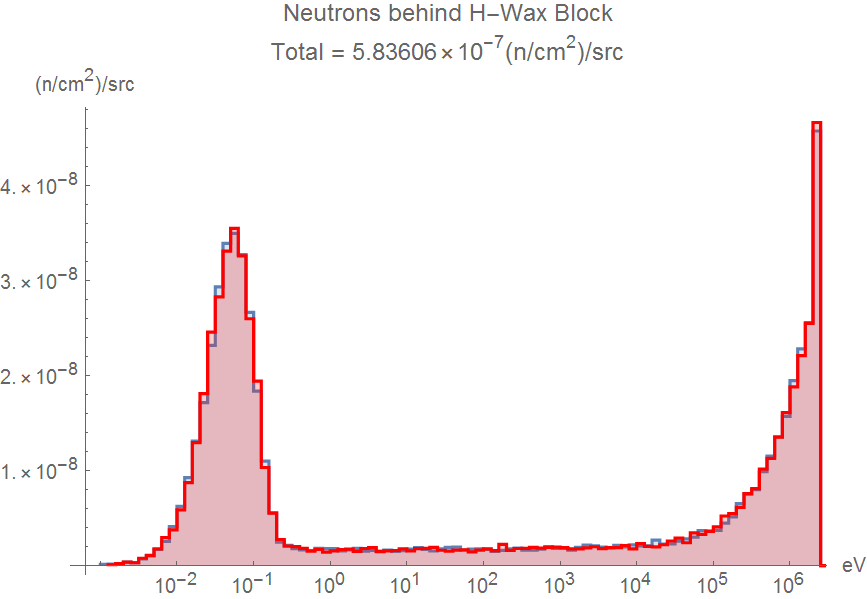
\includegraphics[width=0.7\columnwidth]{sn2304}
	\caption{
		\label{fig.fluence}
		Two fluence histograms that we would like to compare.
	}
\end{figure}

Consider the histograms in figure \ref{fig.fluence}, which show neutron fluence as computed by two different programs. We would like to know if the histograms match as well as they should, given the statistics, or is there some difference between them, as might be seen in the lower (thermal) peak? 

We would take the results of the program that we declare to be the ``gold standard'', in this case MCNP, and use it as our model, and then ask what is the $\chi^2$ when compared to the results of another program.

Our measurements in this case are the fluence values in the histogram bins. Are they independent or correlated? The answer is that they are highly correlated. A single neutron path will contribute fluence to many bins during the simulation. We have seen in detail how neutrons scatter, and we know that when the neutron has low energy it is very likely to scatter into a nearby energy bin. And so counts and fluence in one bin make it likely that neighboring bins also have counts.

Therefore, we need to use equation (\ref{eq.general.chi.square}) to compute the $\chi^2$. The number of degrees of freedom is the number of bins, and we would use the $chi^2$ distribution to determine how well the histograms match.

In order to do this, we need to know the covariance matrix for the measurements in each bin.  Unfortunately, this is a matter of current software development as we cannot calculate the covariance from first principles, and so need to collect it during simulation.

\section{Comparing Distribution Histograms}

\begin{figure}[ht] 
	\centering	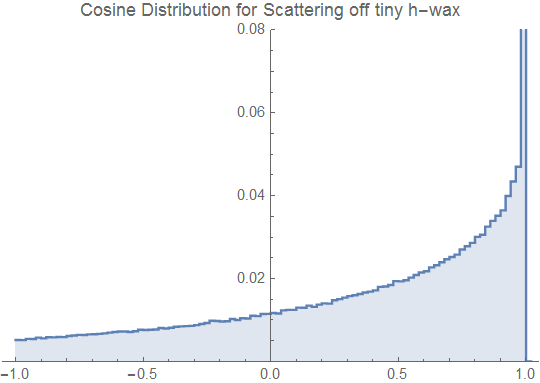
\includegraphics[width=0.7\columnwidth]{CosineDistributionMCNP}
	\caption{
		\label{fig.cosine}
		A histogram showing a probability distribution.
	}
\end{figure}

We also have another kind of histogram to compare that is fundamentally different. In figure \ref{fig.cosine} for example, we have scattered neutrons off of a target and then count them in bins according to the angle of the scattering. This has the nice property that each neutron can contribute only once to the histogram. Each neutron is independent of the next, so does this mean that the bin counts are independent? Interestingly, they are not.

When a neutron is counted in one bin, it is \textit{not} counted in another! This actually means that there is a negative correlation between bin counts. It may be easier to understand when you think of it in terms of a random fluctuation away from the average. Suppose one bin, by pure luck, happens to get more hits than its fair share. Because the total number of particles is fixed, some other bin or bins must be lower than expected.

This differs in a fortunate way from the fluence histogram in that we can calculate the covariance matrix for the bins from first principles. We will not need to collect any extra data to compute the $\chi^2$ for the comparison of two of these histograms.






\end{document}
